\subsection{Halaman User}

Halaman user adalah halaman yang ditujukan untuk pengguna yang ingin melakukan reservasi dan menikmati layanan yang tersedia di Tamu.id.

\subsubsection{Registrasi dan Login User}

Pada halaman pendaftaran user, pengguna dapat melakukan pendaftaran dengan dua metode yaitu dengan mengunakan email atau menggunakan akun google langsung yang membuatnya lebih instan dan mudah. Tampilan halaman pendaftaran user dapat dilihat pada Gambar \ref{fig:halaman-daftar-user}.

\begin{figure}[H]
    \centering
    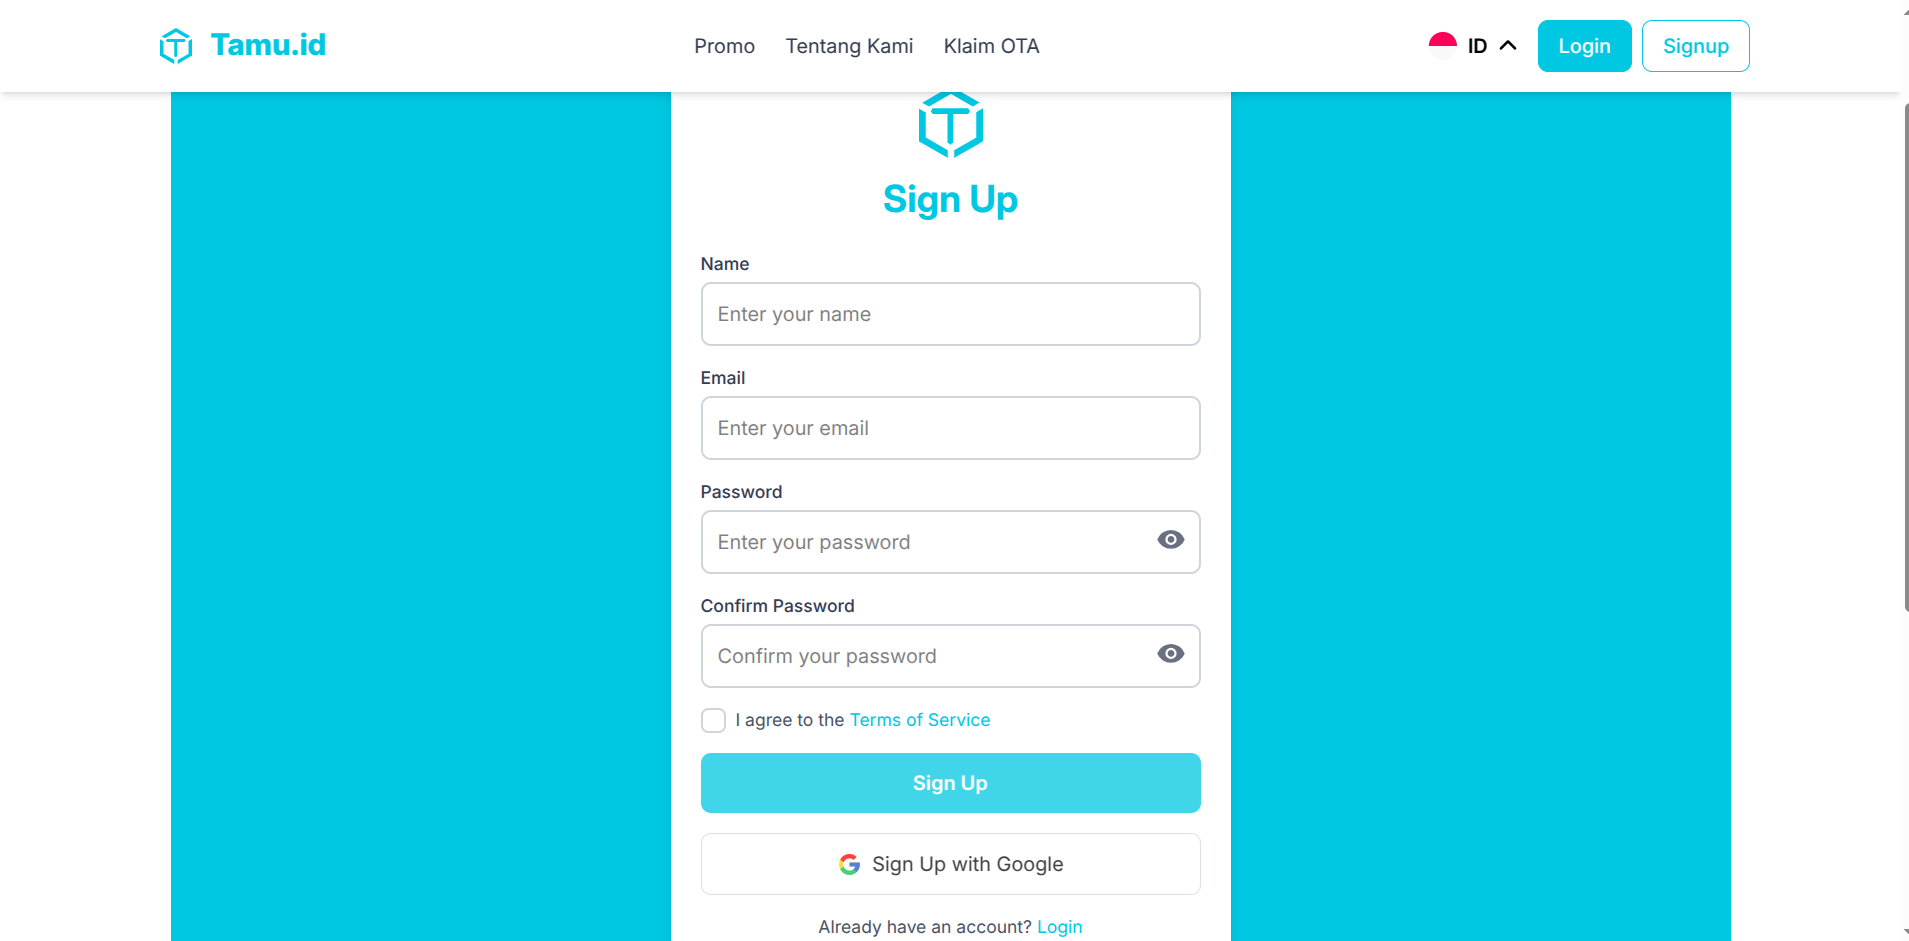
\includegraphics[width=\textwidth]{images/halaman-user/signup.png}
    \caption{Tampilan Halaman Pendaftaran User}
    \label{fig:halaman-daftar-user}
\end{figure}

Setelah pengguna melakukan pendaftaran, pengguna dapat melakukan login ke dalam aplikasi Tamu.id. Tampilan halaman login user dapat dilihat pada Gambar \ref{fig:halaman-login-user}.

\begin{figure}[H] % Pertimbangkan [htbp] untuk penempatan float yang lebih fleksibel
    \centering
    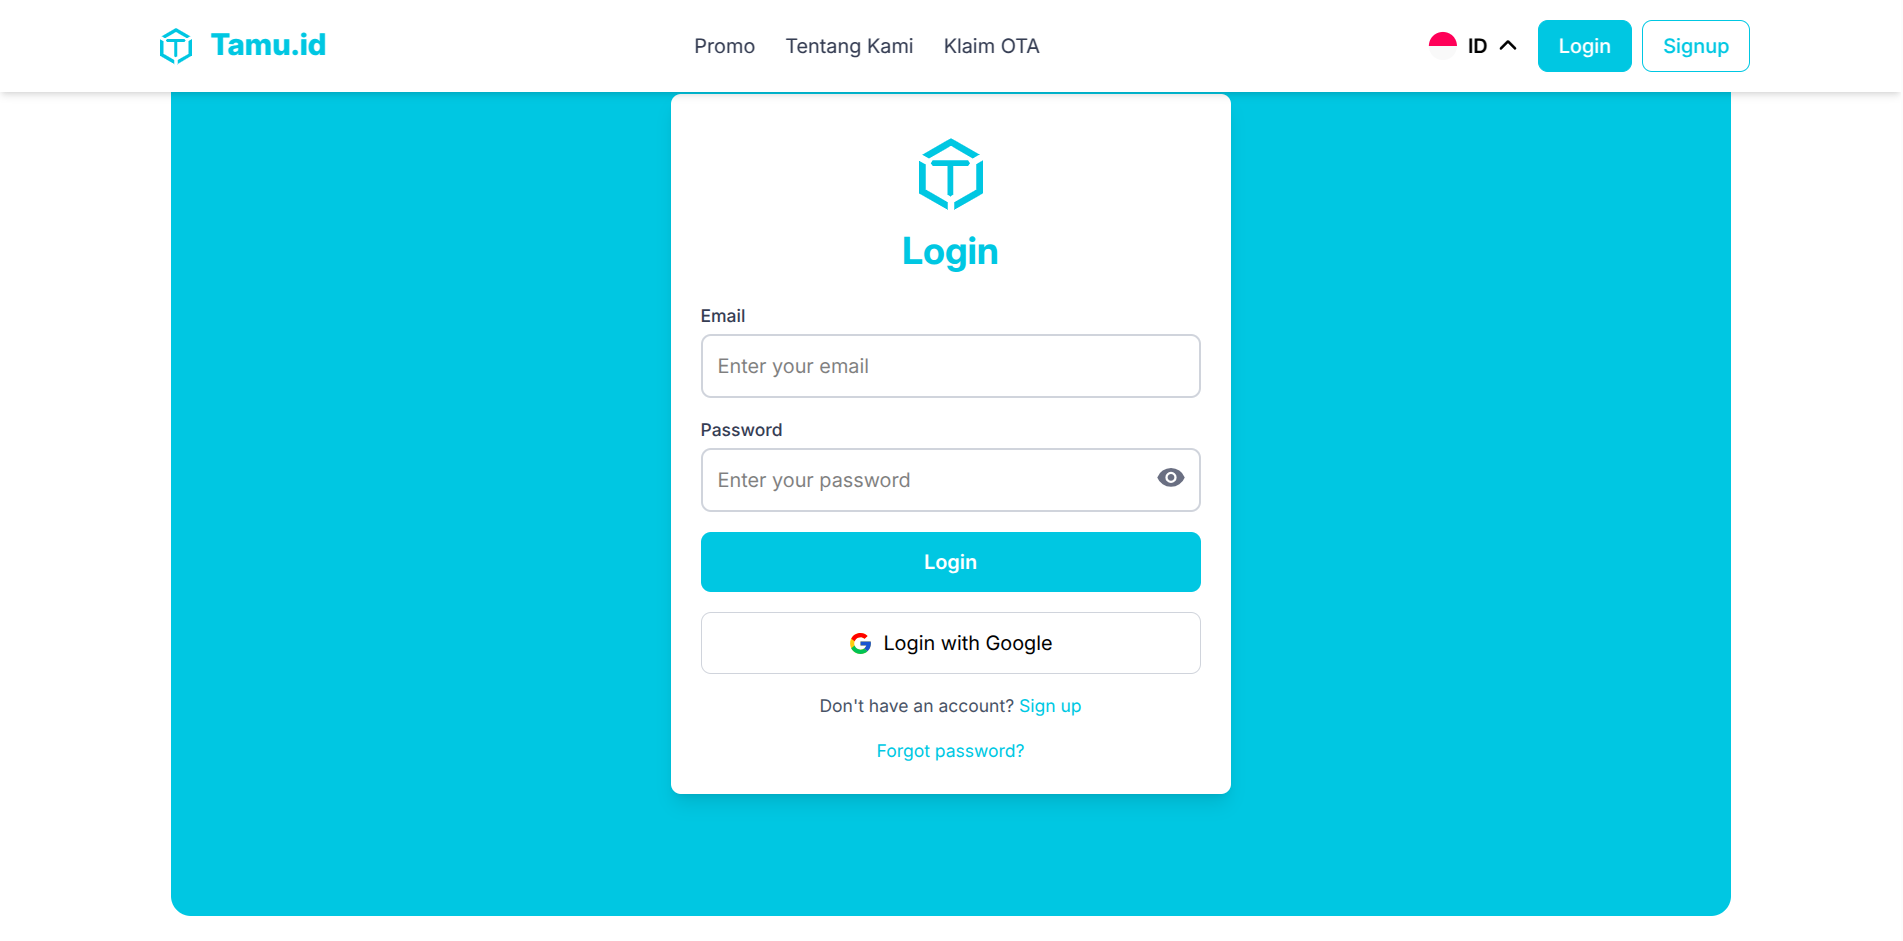
\includegraphics[
        width=1.0\textwidth, % Atur lebar sesuai kebutuhan, misal 90% lebar teks
        keepaspectratio % Opsi ini biasanya implisit atau dikelola dengan baik oleh width
    ]{images/halaman-user/login.png} % Path ke file SVG Anda, TANPA ekstensi .svg
    \caption{Tampilan Halaman Login User}
    \label{fig:halaman-login-user}
\end{figure}

Pada kode \ref{lst:fe-login-user} berikut adalah implementasi frontend untuk halaman login dan pendaftaran user. Kode ini mengatur tampilan dan interaksi pengguna untuk proses login dan pendaftaran.

\lstinputlisting[
    language=VUE,
    caption={Implementasi Frontend Login User},
    label={lst:fe-login-user},
]{codes/user/login/login.vue}


Salah satu fitur utama yaitu integrasi dengan Oauth Google yang memungkinkan pengguna untuk masuk ke aplikasi menggunakan akun Google mereka. Hal ini memberikan kemudahan bagi pengguna yang tidak ingin mengingat password tambahan. Implementasi fitur ini dapat dilihat pada kode \ref{lst:be-google-signin}.

\lstinputlisting[
    language=Python,
    caption={Implementasi Oauth Google pada Halaman Login dan Sign Up User},
    label={lst:be-google-signin},
]{codes/user/login/login-google.py}

\subsubsection{Landing Page User}

Landing page adalah halaman utama yang ditampilkan kepada pengguna dalam sistem. Halaman ini memberikan informasi umum tentang layanan yang tersedia, termasuk fitur-fitur utama, manfaat, dan cara menggunakan aplikasi.

\begin{figure}[H]
    \centering
    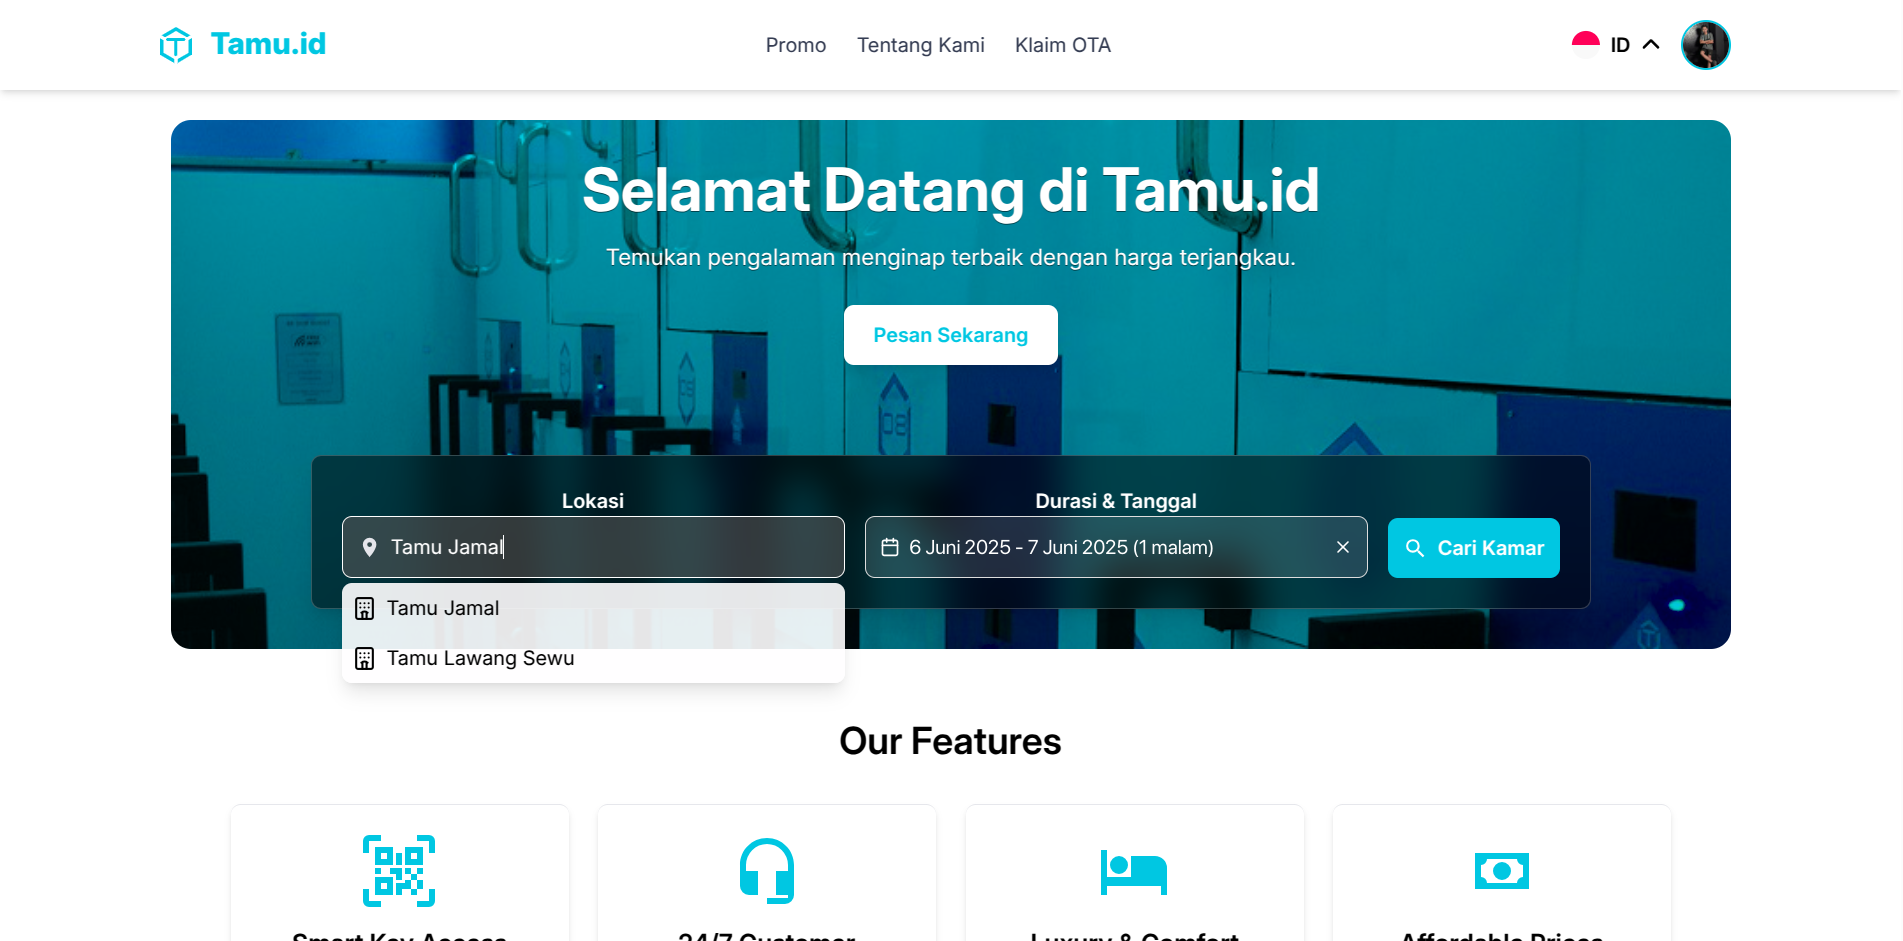
\includegraphics[width=\textwidth]{images/halaman-user/home.png}
    \caption{Tampilan Halaman Landing Page User}
    \label{fig:halaman-landing-user}
\end{figure}

Pada gambar \ref{fig:halaman-landing-user}, terlihat bahwa halaman ini dirancang untuk memberikan pengalaman pengguna yang intuitif dan menarik. Halaman ini dapat diakses oleh pengguna yang telah melakukan login maupun yang belum, sehingga memberikan fleksibilitas dalam penggunaan aplikasi.

\lstinputlisting[
    language=VUE,
    caption={Implementasi Frontend Landing Page User},
    label={lst:fe-landing-user},
]{codes/user/landing/landing.vue}

Pada kode \ref{lst:fe-landing-user}, implementasi frontend untuk landing page user ditampilkan. Dapat terlihat dengan menggunakan Vue.js kita dapat memecah halaman menjadi komponen-komponen yang lebih kecil, sehingga memudahkan pengelolaan dan pengembangan aplikasi.

\subsubsection{Proses Reservasi User}

Halaman reservasi adalah salah satu fitur utama dalam aplikasi yang memungkinkan pengguna untuk melakukan reservasi Pod yang tersedia secara online.

\lstinputlisting[
    language=VUE,
    caption={Implementasi Komponen Pencarian untuk Reservasi},
    label={lst:fe-reservasi-user-search},
]{codes/user/reservation/search.vue}

Kode \ref{lst:fe-reservasi-user-search} menunjukkan implementasi komponen pencarian untuk reservasi. Komponen ini memungkinkan pengguna untuk mencari keterseiaan Pod pada tanggal dan cabang tertentu. Pengguna dapat memasukkan tanggal dan cabang yang diinginkan, dan sistem akan menampilkan daftar Pod yang tersedia untuk reservasi pada tanggal tersebut.


\begin{figure}[H]
    \centering
    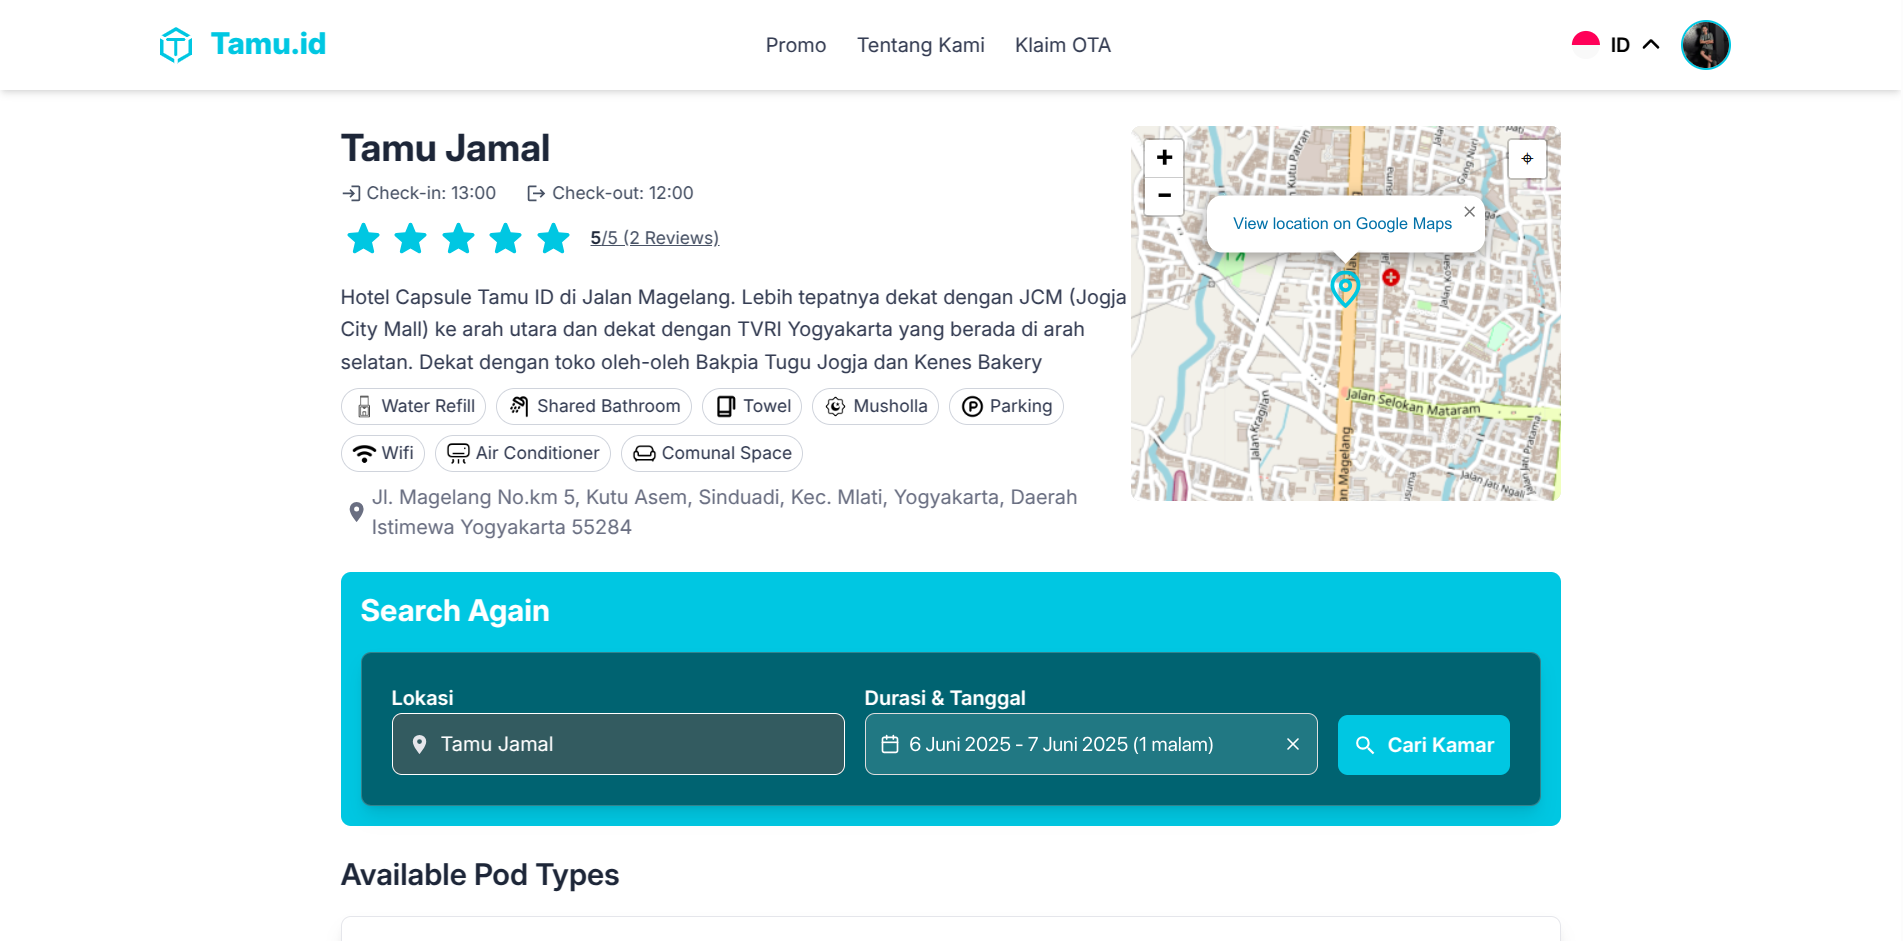
\includegraphics[width=\textwidth]{images/halaman-user/sr2.png}
    \caption{Komponen Pencarian User}
    \label{fig:komponen-pencarian-user}
\end{figure}

Pada gambar \ref{fig:komponen-pencarian-user}, terlihat bahwa komponen pencarian ini dirancang untuk memberikan kemudahan bagi pengguna dalam mencari Pod yang sesuai dengan kebutuhan mereka. Pengguna dapat memilih tanggal dan cabang yang diinginkan

\begin{figure}[H]
    \centering
    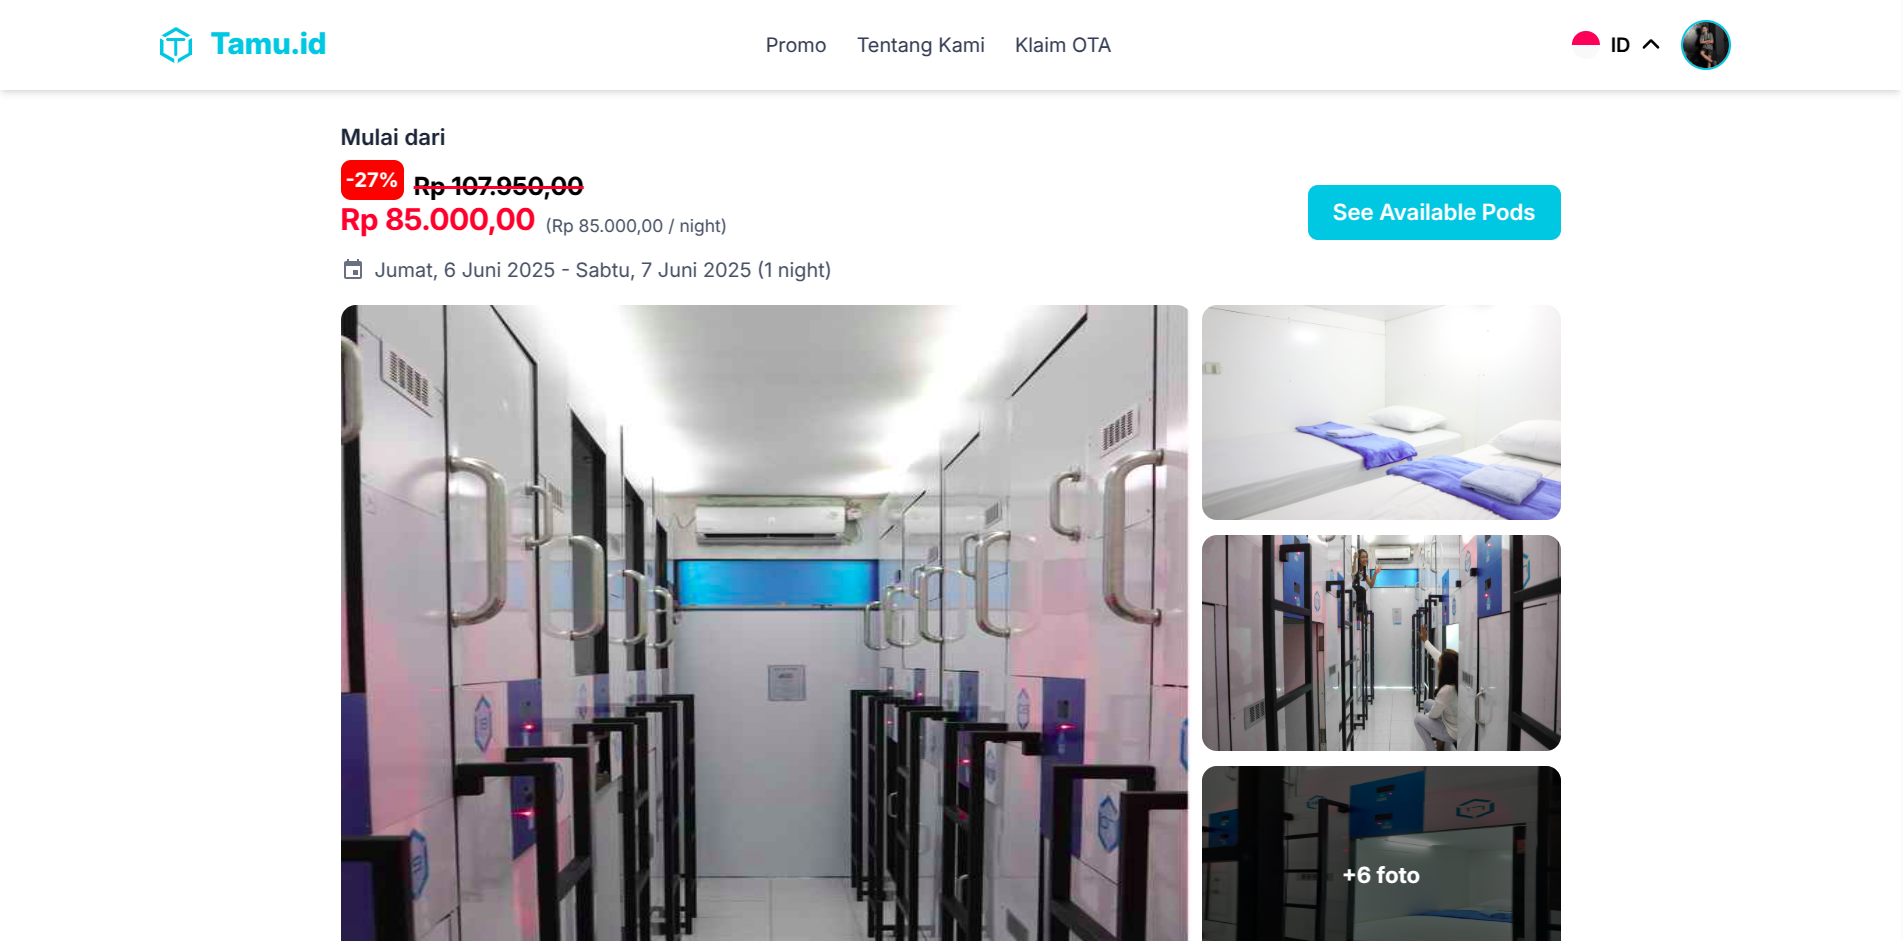
\includegraphics[width=\textwidth]{images/halaman-user/sr.png}
    \caption{Tampilan Hasil Pencarian User}
    \label{fig:hasil-pencarian-user}
\end{figure}

\begin{figure}[H]
    \centering
    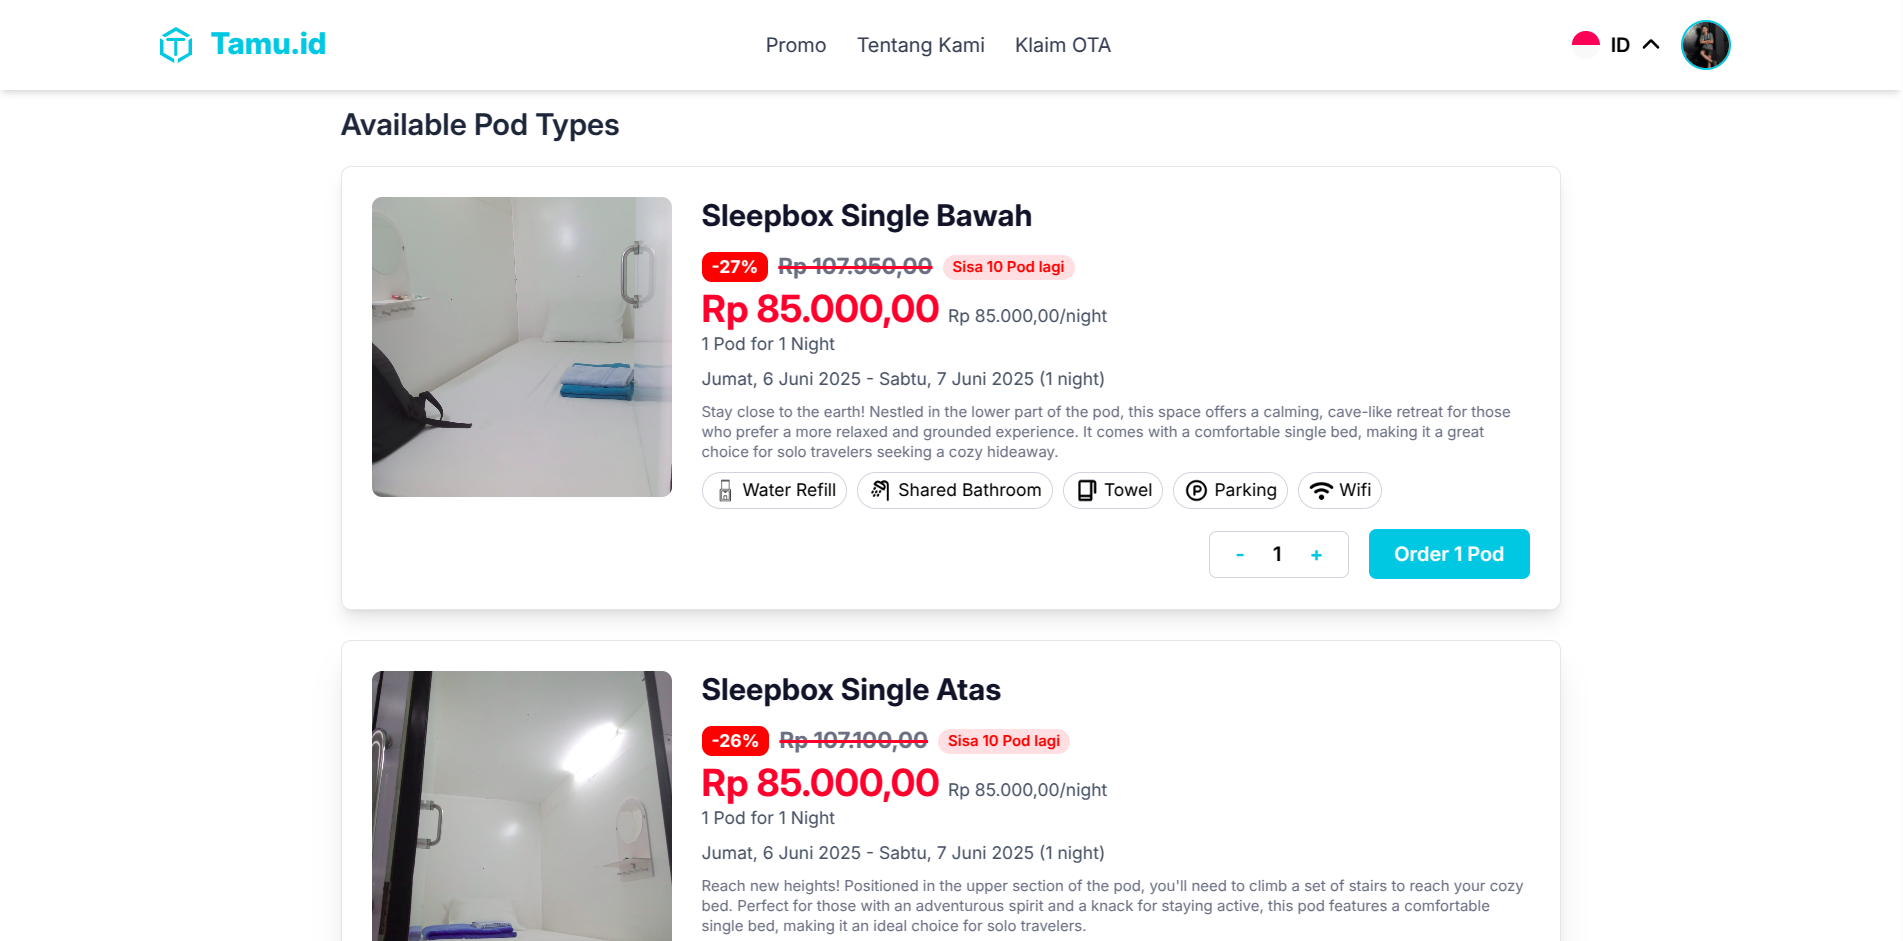
\includegraphics[width=\textwidth]{images/halaman-user/sr3.png}
    \caption{Tampilan Hasil Pencarian User}
    \label{fig:komponen-pencarian-user-2}
\end{figure}

Pada gambar \ref{fig:hasil-pencarian-user} dan \ref{fig:komponen-pencarian-user-2}, terlihat bahwa setelah pengguna memasukkan tanggal dan cabang yang diinginkan, sistem akan menampilkan daftar Pod yang tersedia untuk reservasi pada tanggal tersebut. Pengguna dapat memilih Pod yang diinginkan dan melanjutkan ke proses reservasi.

\begin{figure}[H]
    \centering
    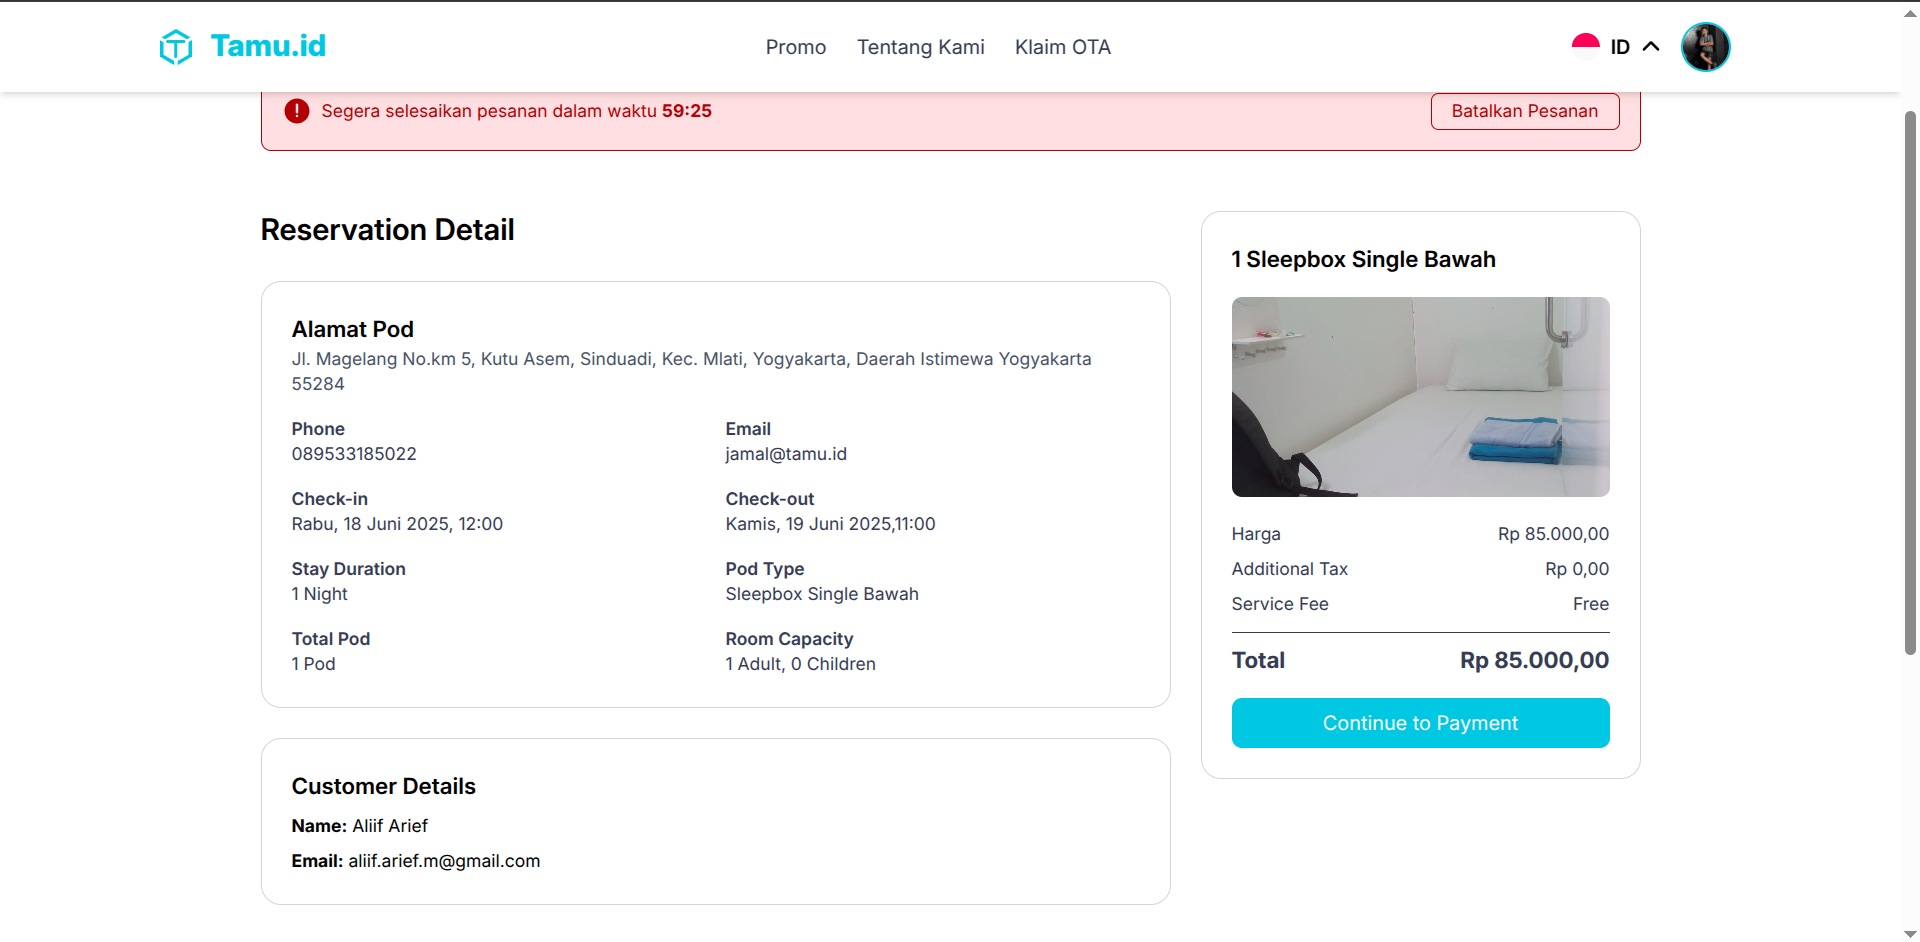
\includegraphics[width=\textwidth]{images/halaman-user/res1.png}
    \caption{Tampilan Proses Pembayaran detail Reservasi}
    \label{fig:tampilan-reservasi-user}
\end{figure}

Setelah pengguna memilih Pod yang diinginkan, maka akan lanjut ke halaman pembayaran yang terdiri dari tiga proses yaitu pada gambar \ref{fig:tampilan-reservasi-user} merupakan proses pertama pengguna dapat melihat detail reservasi yang dia lakukan.

\begin{figure}[H]
    \centering
    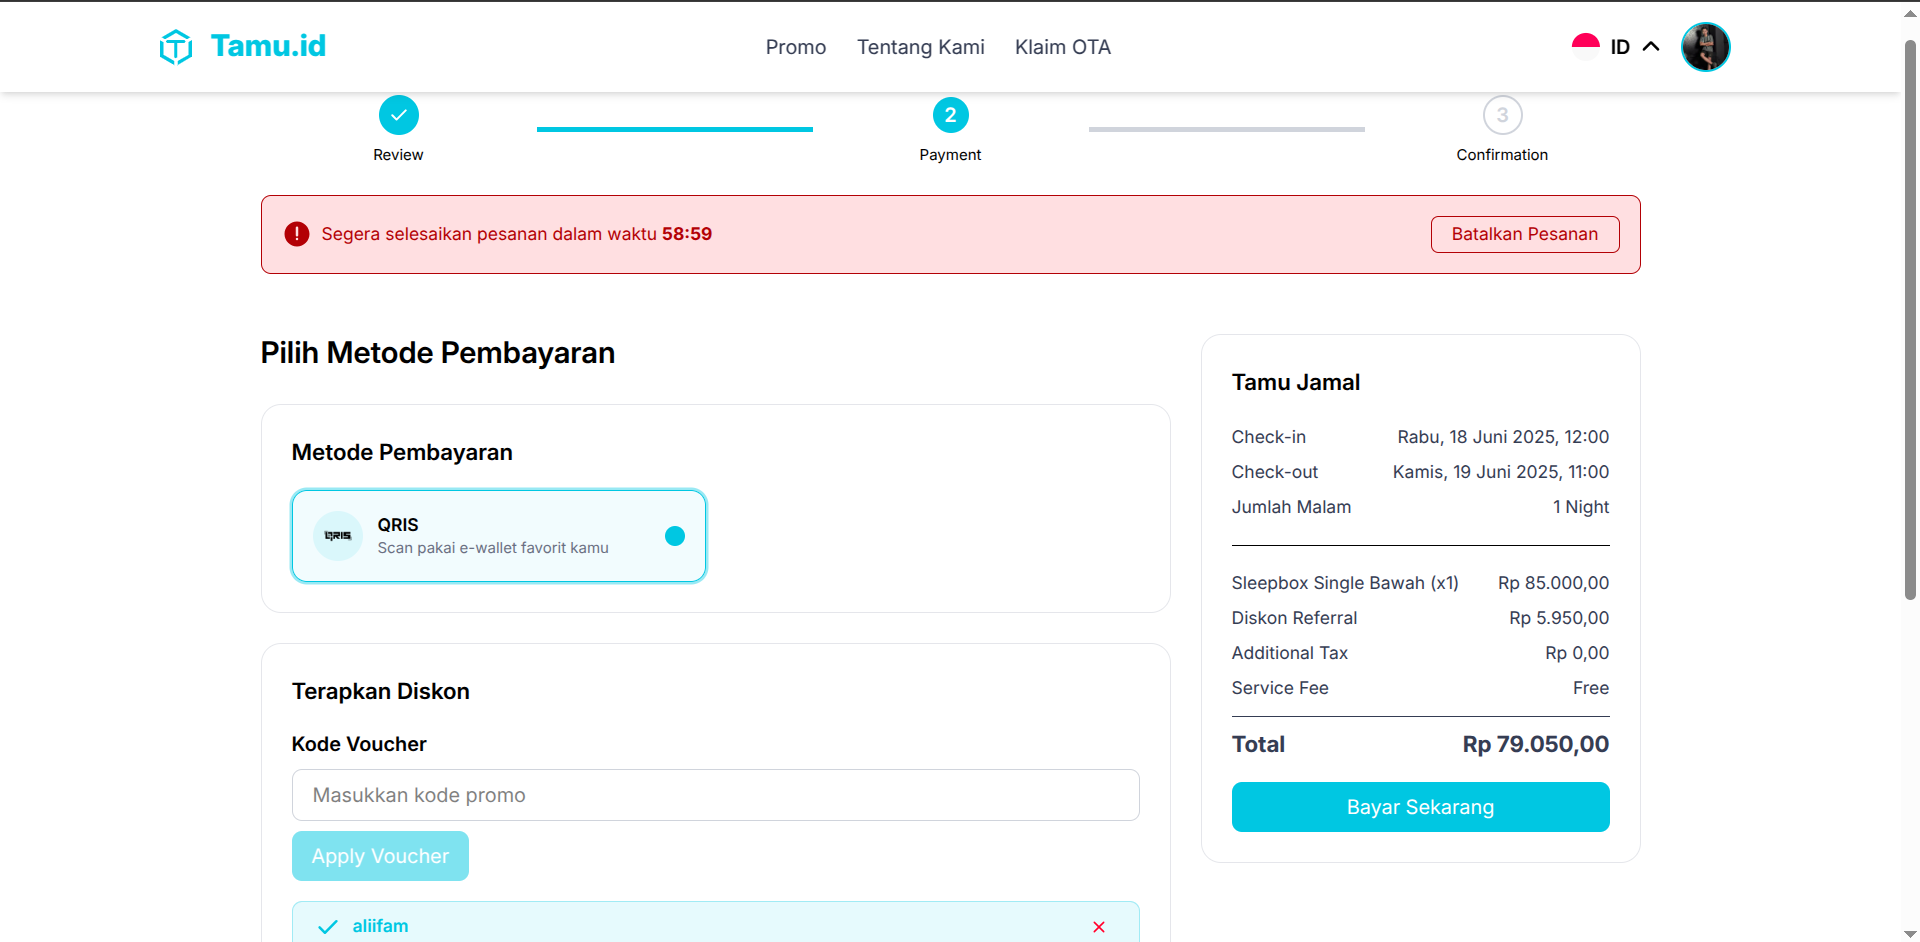
\includegraphics[width=\textwidth]{images/halaman-user/res2.png}
    \caption{Tampilan Proses Pembayaran Metode Pembayaran}
    \label{fig:tampilan-reservasi-user-2}
\end{figure}

Pada gambar \ref{fig:tampilan-reservasi-user-2}, pengguna dapat memilih metode pembayaran yang diinginkan yaitu QRIS lalu dalam tahap ini pengguna dapat memasukkan kode voucher dan kode referral untuk mendapatkan potongan harga.

\begin{figure}[H]
    \centering
    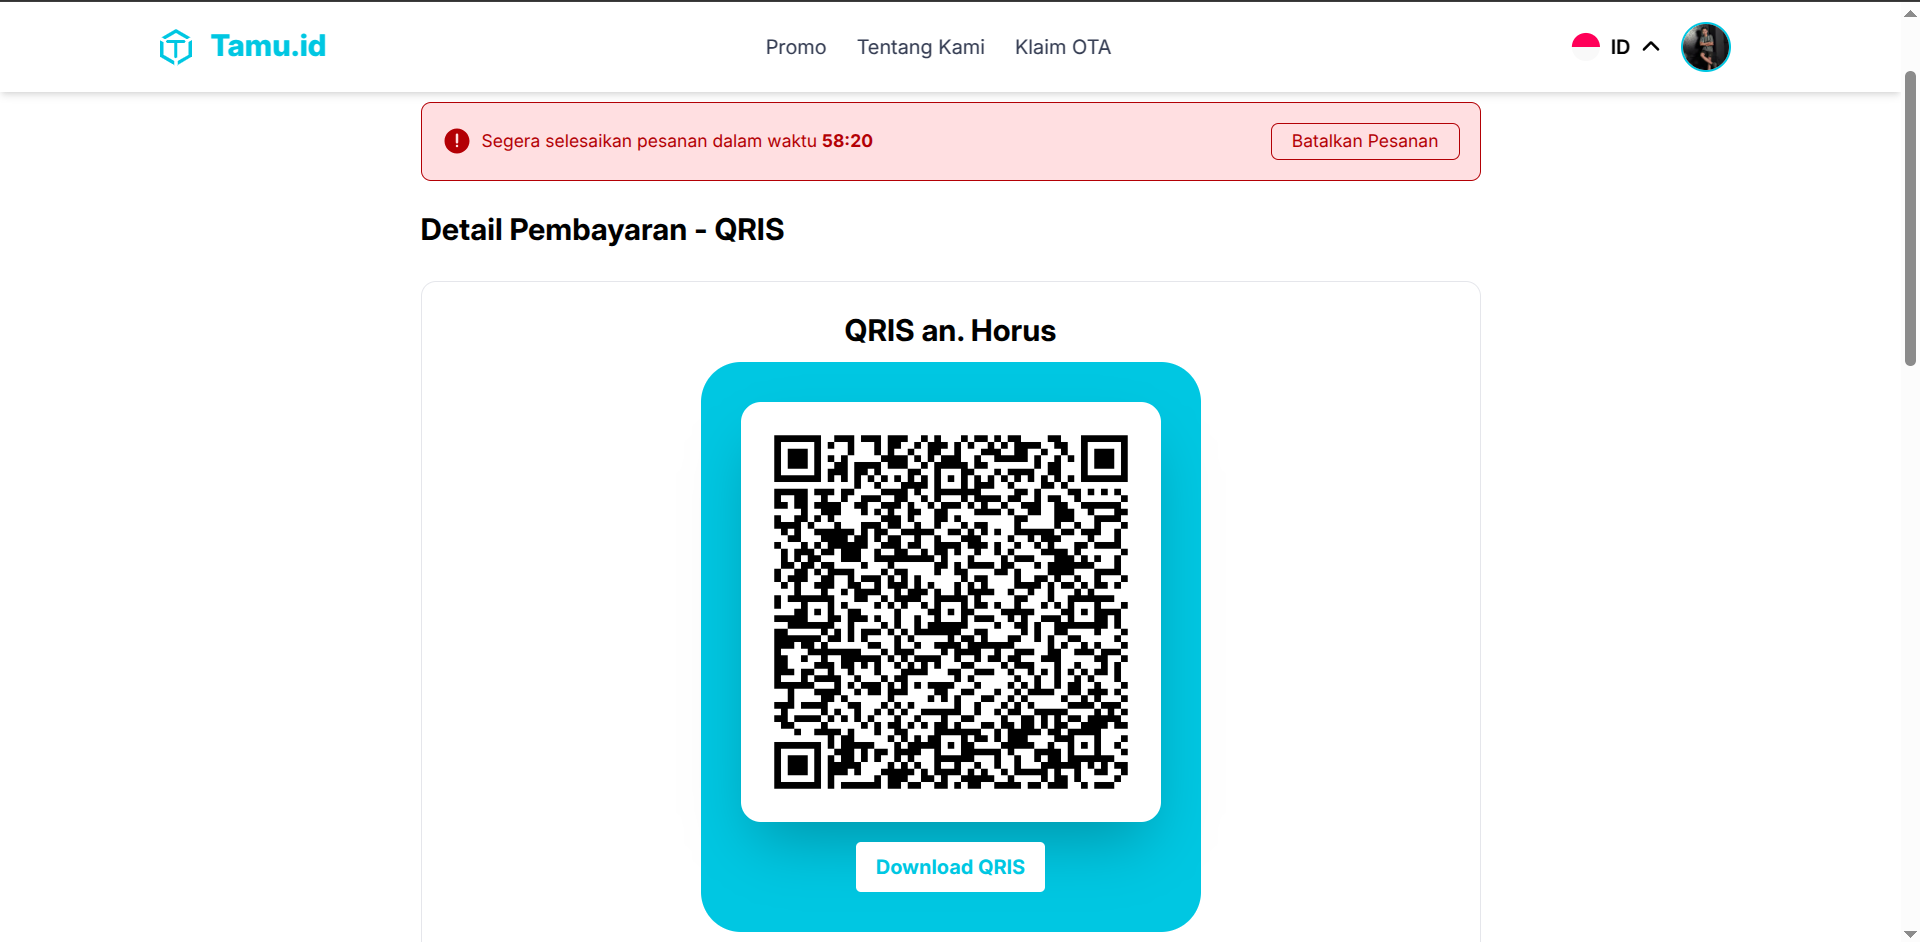
\includegraphics[width=\textwidth]{images/halaman-user/res3.png}
    \caption{Tampilan Proses Pembayaran kode QRIS}
    \label{fig:tampilan-reservasi-user-3}
\end{figure}

\begin{figure}[H]
    \centering
    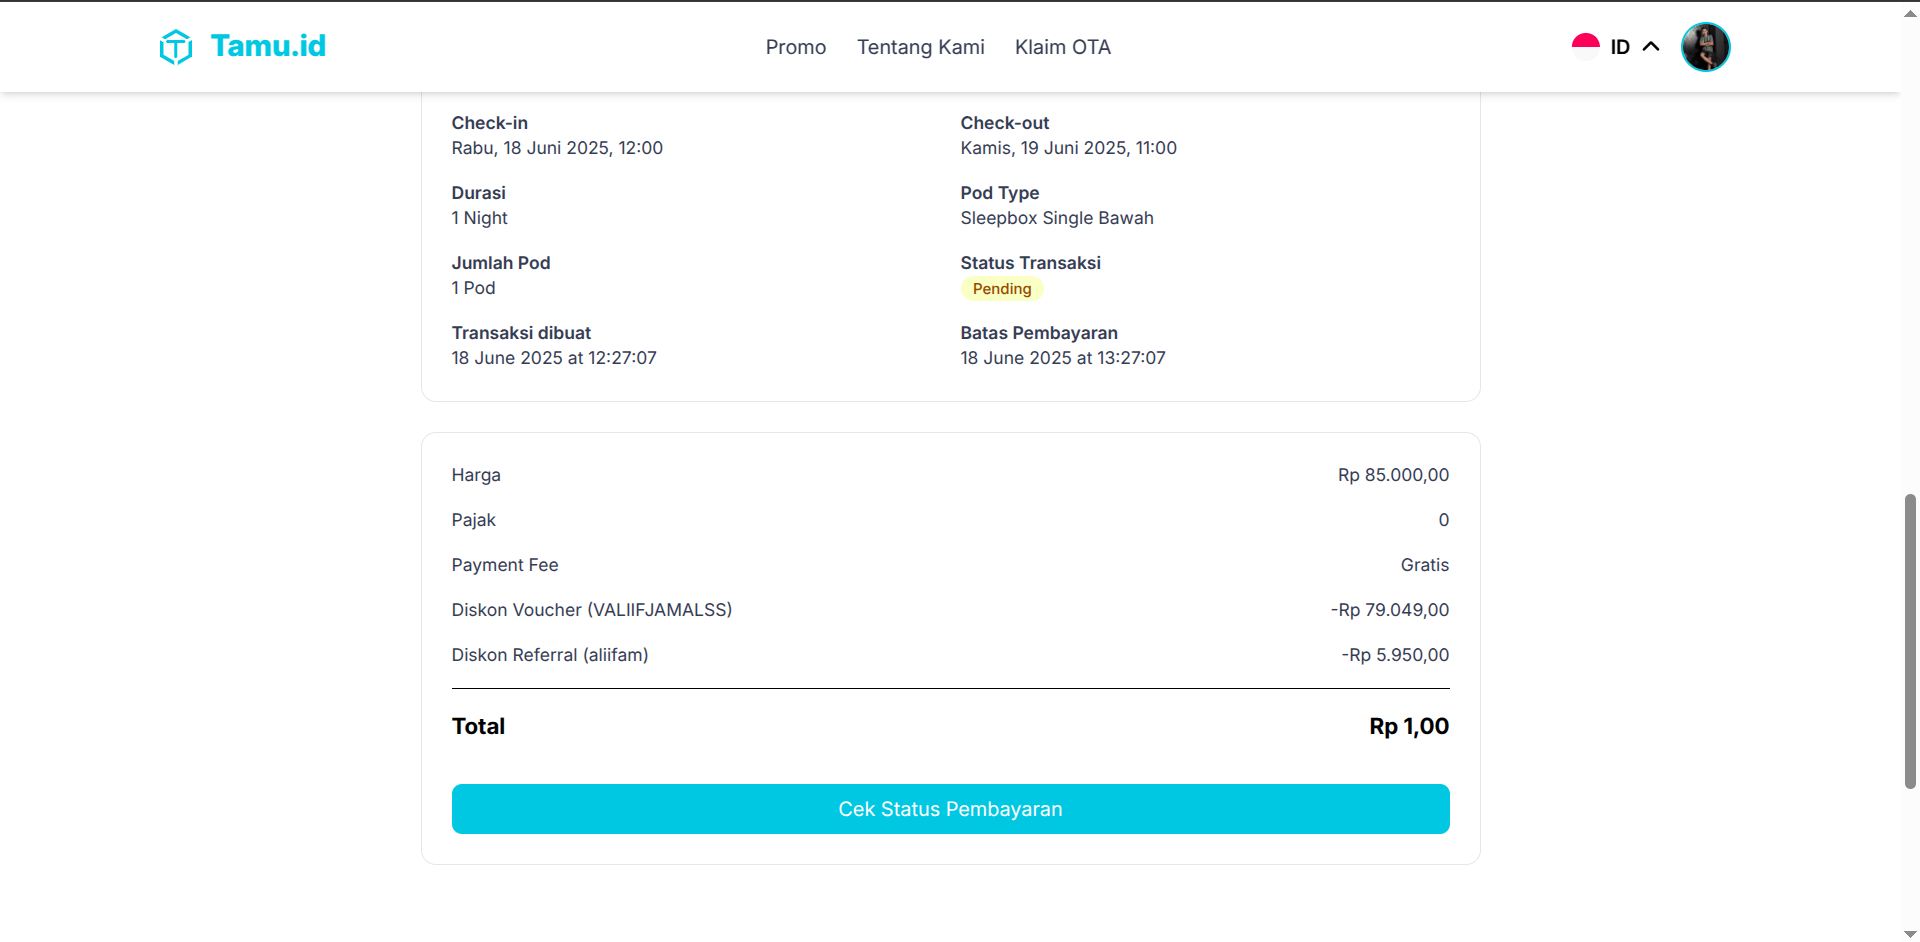
\includegraphics[width=\textwidth]{images/halaman-user/res4.png}
    \caption{Tampilan Proses Pembayaran \textit{Pending}}
    \label{fig:tampilan-reservasi-user-4}
\end{figure}

Pada gambar \ref{fig:tampilan-reservasi-user-3} dan \ref{fig:tampilan-reservasi-user-4} setelah itu sistem akan terhubung dengan \textit{payment gateway} dan menampilkan kode QRIS yang dapat di scan oleh pengguna untuk melakukan pembayaran.

\begin{figure}[H]
    \centering
    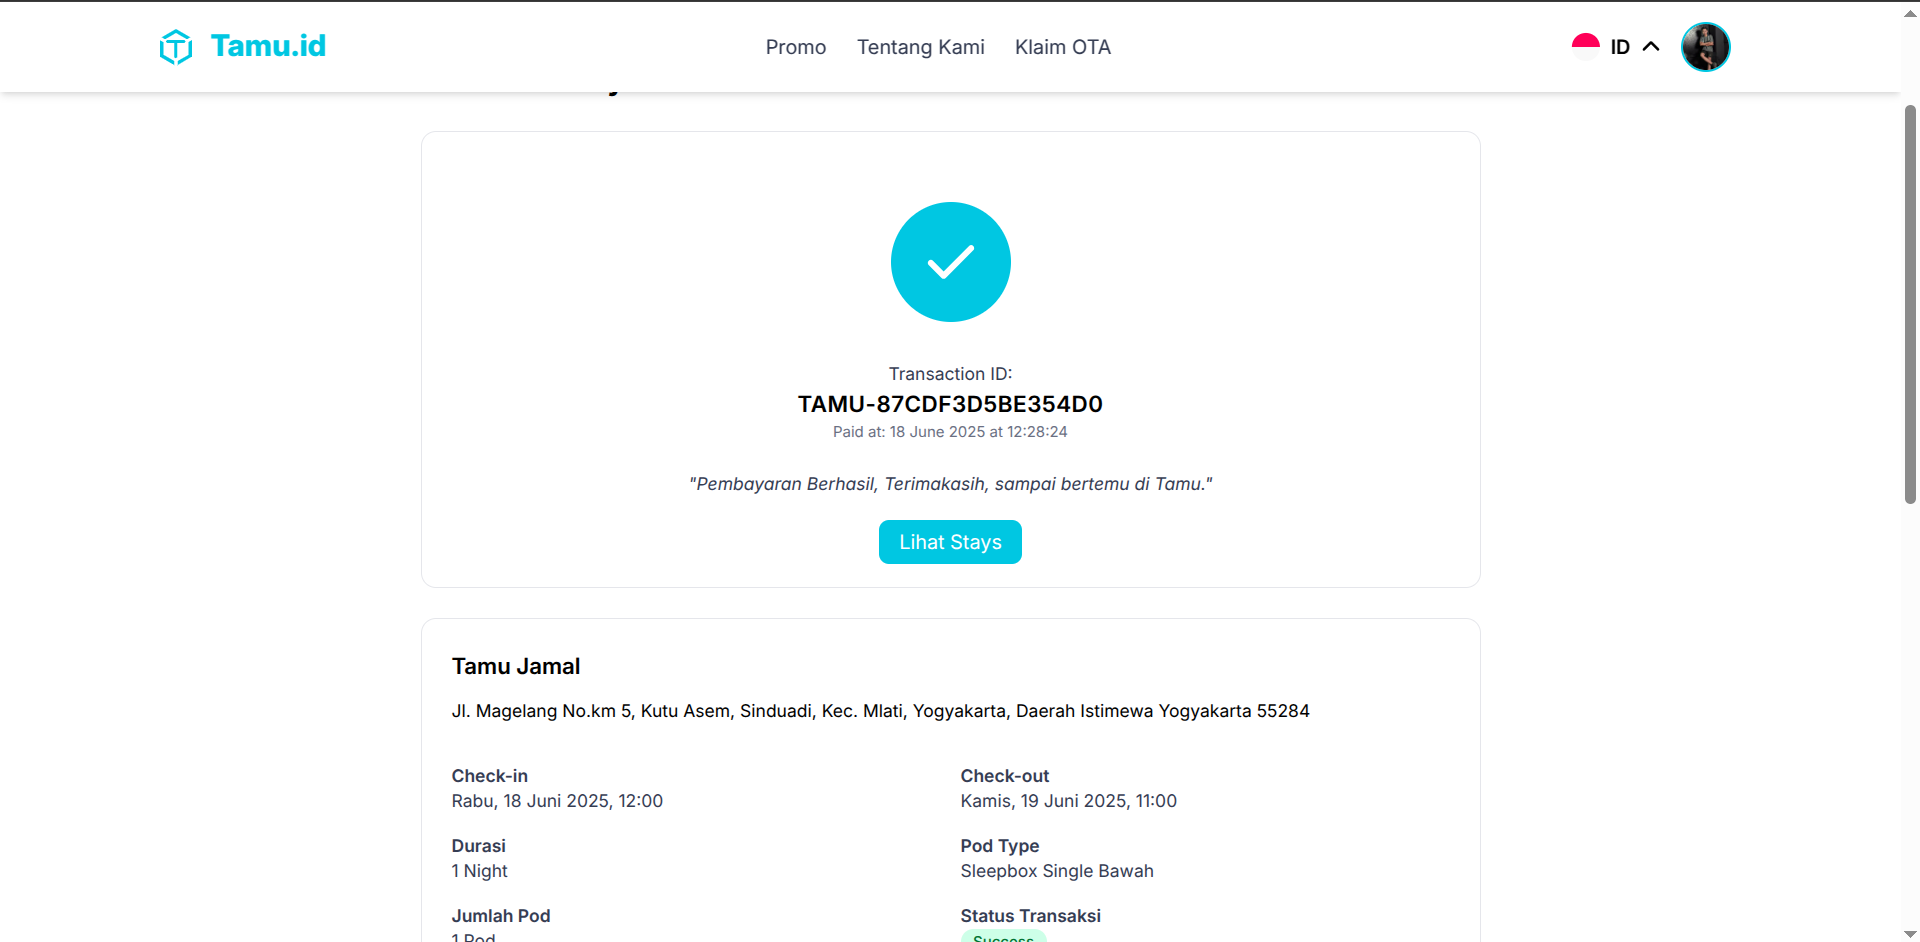
\includegraphics[width=\textwidth]{images/halaman-user/res5.png}
    \caption{Tampilan Proses Pembayaran \textit{Success}}
    \label{fig:tampilan-reservasi-user-5}
\end{figure}

Setelah pengguna melakukan pembayaran, maka akan muncul halaman konfirmasi bahwa reservasi berhasil dilakukan. Pengguna dapat melihat detail reservasi yang telah dilakukan pada gambar \ref{fig:tampilan-reservasi-user-5}.


\subsubsection{Proses Menginap User}

Setelah melakukan reservasi tentunya pengguna akan menginap di jenis Pod yang telah dipesan, berikut proses yang dilakukan oleh pengguna ketika menginap di Pod yang telah dipesan.

\begin{figure}[H]
    \centering
    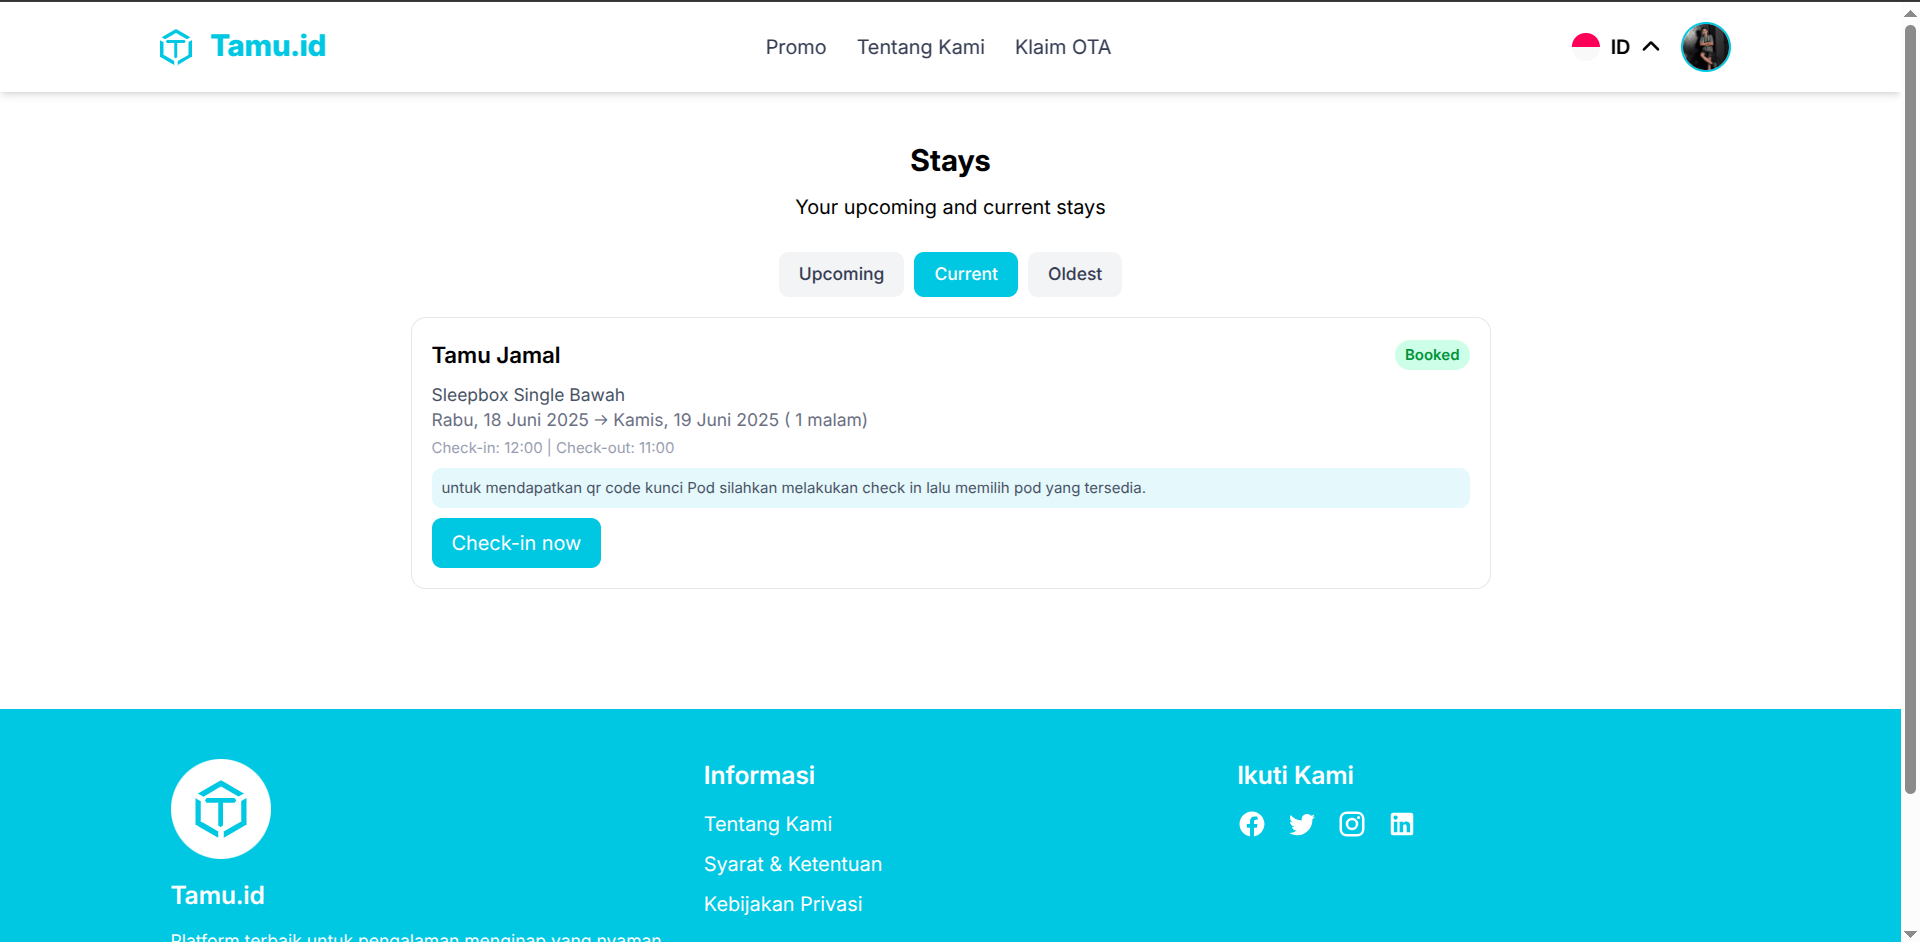
\includegraphics[width=\textwidth]{images/halaman-user/stay1.png}
    \caption{Tampilan List Reservasi User}
    \label{fig:tampilan-list-reservasi-user}
\end{figure}

Pada gambar \ref{fig:tampilan-list-reservasi-user}, pengguna dapat melihat daftar reservasi yang telah dilakukan, terdiri dari tiga status yaitu \textit{upcoming}, \textit{current}, dan \textit{oldest}. Pengguna dapat melakukan check-in pada reservasi yang berstatus \textit{current} yaitu reservasi yang waktu check-in sudah tiba. Pengguna dapat melakukan check-in dengan menekan tombol \textit{Check In} pada reservasi yang berstatus \textit{current}.

\begin{figure}[H]
    \centering
    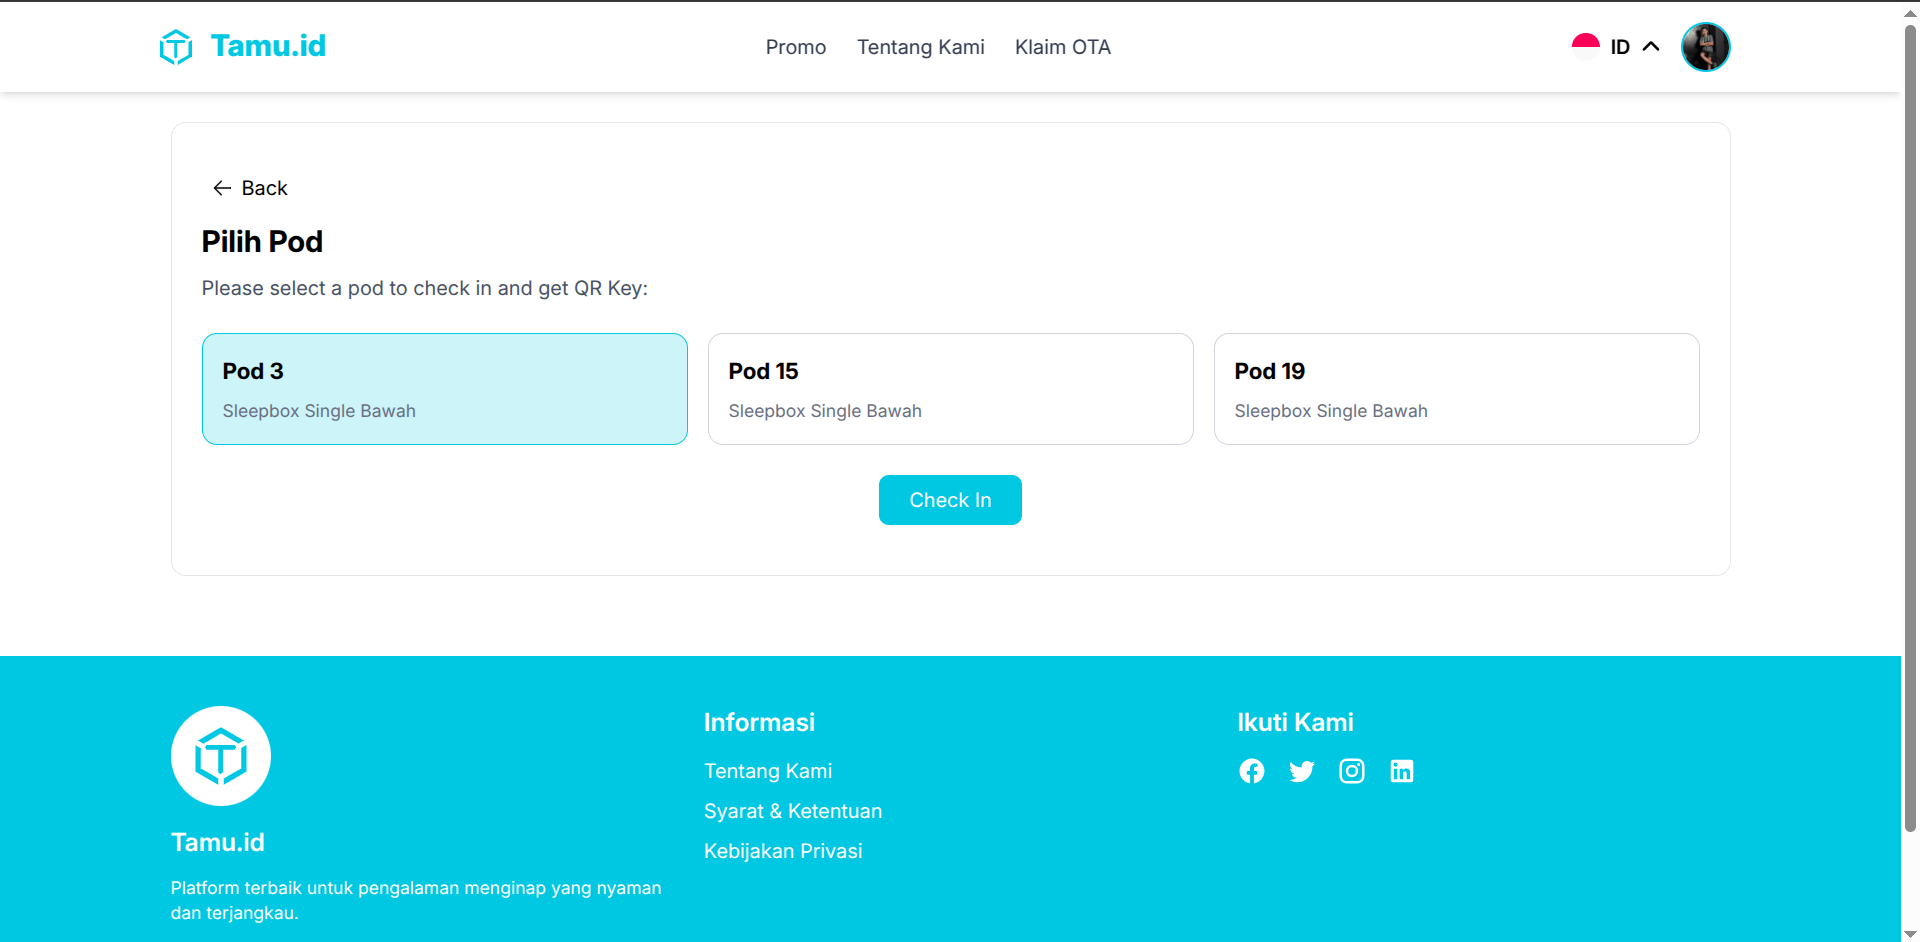
\includegraphics[width=\textwidth]{images/halaman-user/stay2.png}
    \caption{Tampilan Proses pilih Pod User}
    \label{fig:tampilan-pick-a-pod-user}
\end{figure}

Setelah klik tombol \textit{Check In}, pengguna akan diarahkan ke halaman \ref{fig:tampilan-pick-a-pod-user} untuk memilih Pod yang akan ditempati. Pengguna dapat memilih Pod yang diinginkan dan melanjutkan ke proses check-in.

\begin{figure}[H]
    \centering
    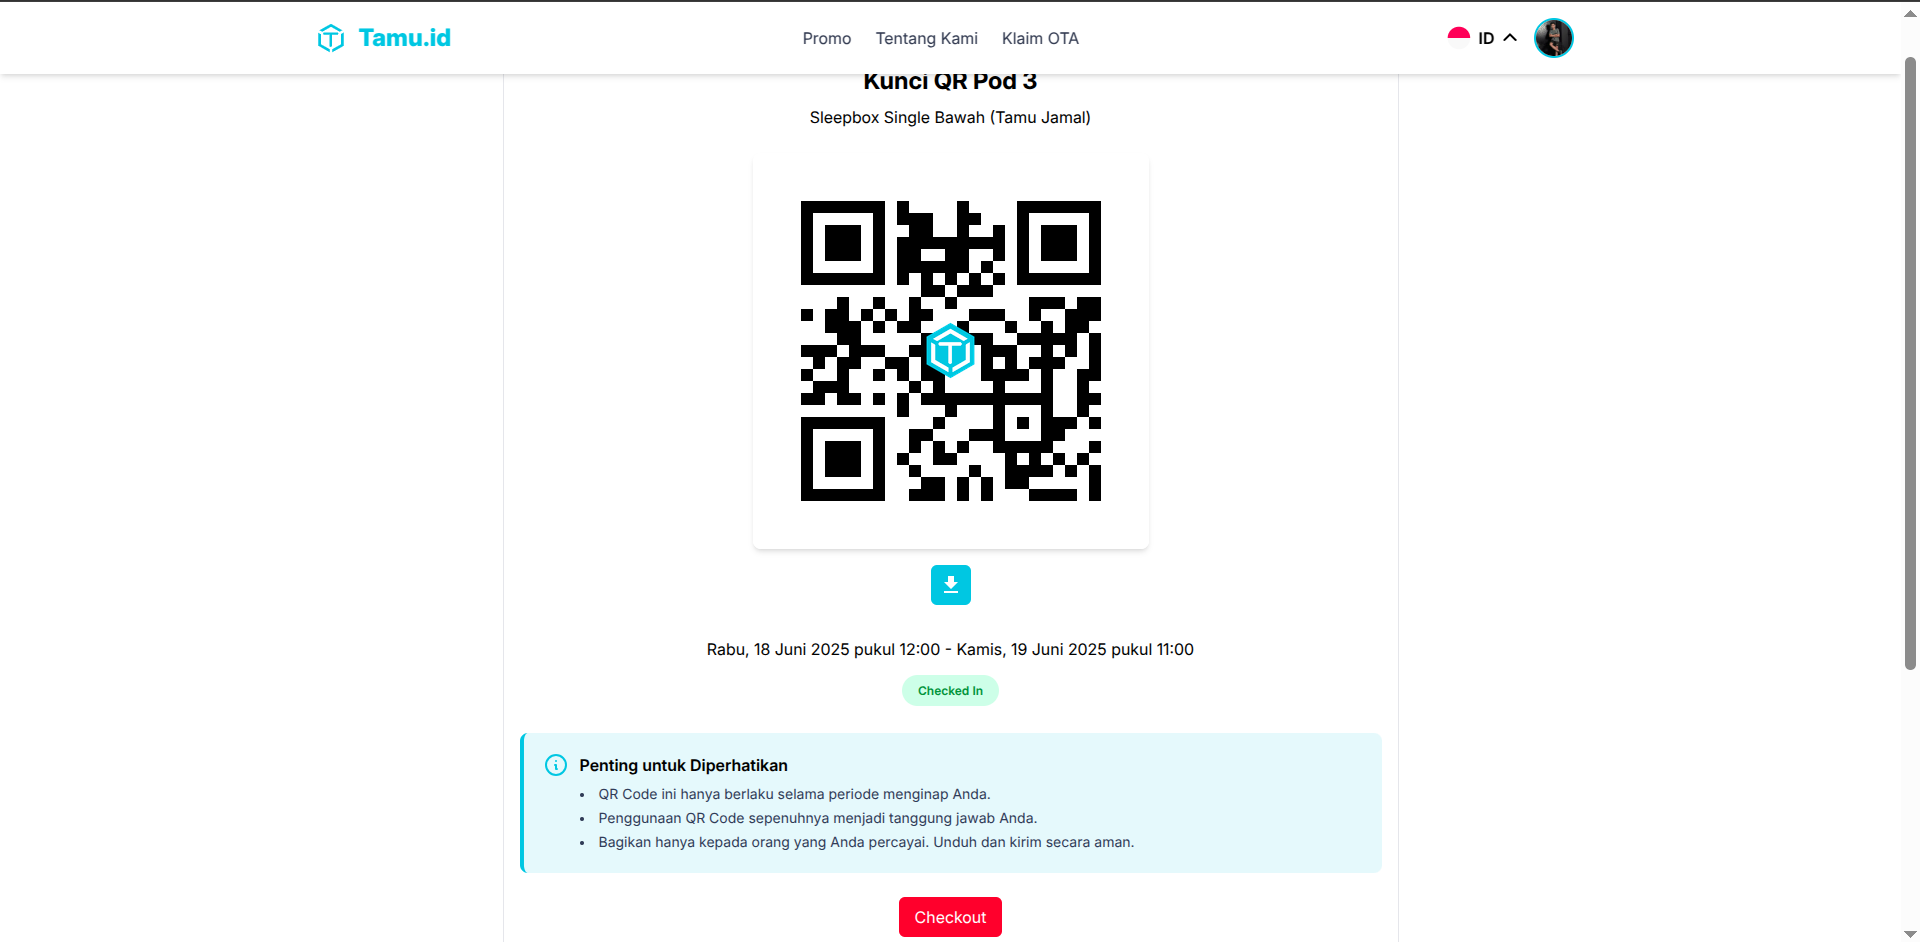
\includegraphics[width=\textwidth]{images/halaman-user/stay3.png}
    \caption{Tampilan Kunci Pod User}
    \label{fig:tampilan-lock-pod-user}
\end{figure}

Setelah memilih Pod yang diinginkan, pengguna akan diarahkan ke halaman \ref{fig:tampilan-lock-pod-user} dan mendapatkan kunci Pod yang telah dipilih yang kuncinya merupakan QR Code yang dapat di scan oleh pengguna untuk membuka Pod yang telah dipilih.

\begin{figure}[H]
    \centering
    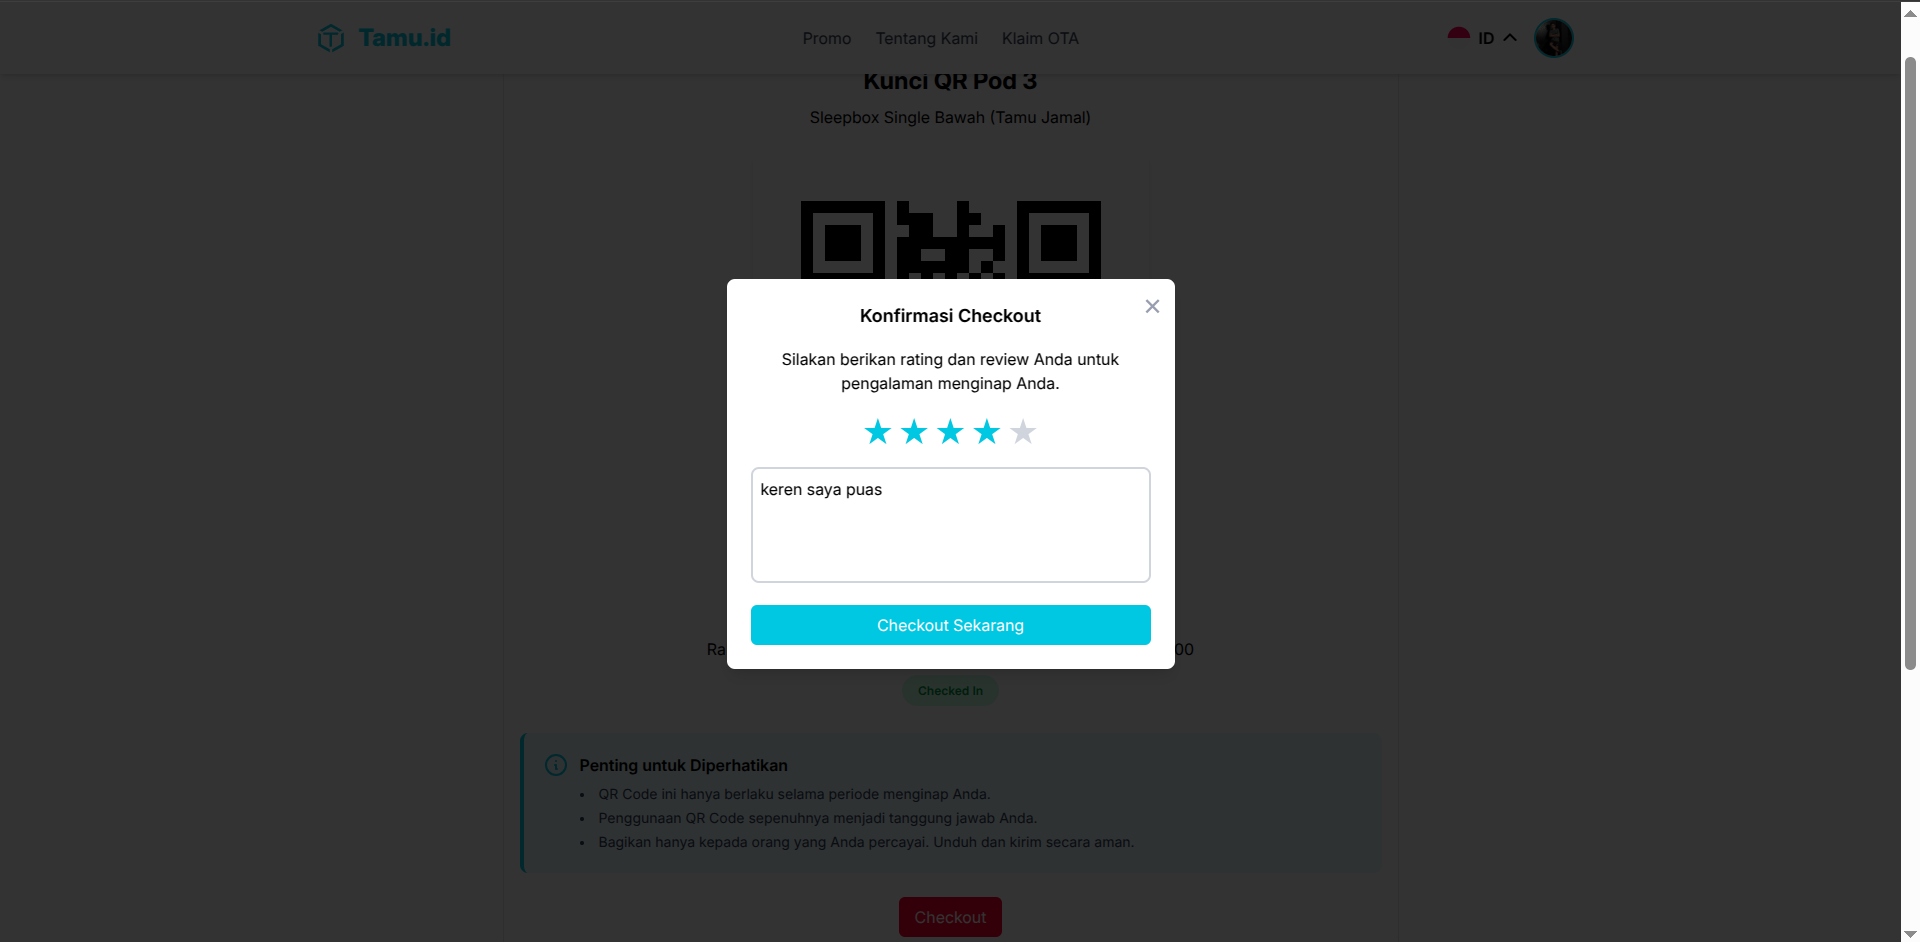
\includegraphics[width=\textwidth]{images/halaman-user/stay4.png}
    \caption{Tampilan Checkout dan Memberikan Ulasan User}
    \label{fig:tampilan-checkout-user}
\end{figure}

Setelah pengguna selesai menginap, maka pengguna dapat melakukan checkout dengan menekan tombol \textit{Checkout} pada gambar \ref{fig:tampilan-checkout-user}. Setelah itu pengguna dapat memberikan ulasan terhadap Pod yang telah ditempati. Ulasan ini akan membantu pengguna lain dalam memilih Pod yang sesuai dengan kebutuhan mereka.
